\section{Introduction}

% object model is critical
All data is presented as object in mainstream dynamic languages like Python, Ruby and JavaScript.
Programs written in those languages interact with data using objects.
Object model, the implementation behind the object representation is a core component of a language runtime implementation.
Not only it has to be efficient for accessing the reperesented data, it also needs to respect the dynamic nature of those languages.
An efficient dynamic language implementation should handled object modifications at runtime in less expensive ways.

% hosted language is the trend
Despite their popularity, performance has been the weakness of dynamic languages.
Languages like Python and Ruby are originally implemented as interpreters.
Although interpreters are easy to implement, their performance is suboptimal.
To address this weakness, we have seen previous works that have improved the performance of dynamic languages
by constructing a complete just-in-time (JIT) compilation based virtual machine for one particular language.
This approach offers promising performance benefit, but incurs significant implementation costs.

Alternatively, language implementors can build their languages on top of an existing mature virtual machine such as the Java Virtual machine (JVM).
In this way, the ``guest'' language can reuse the existing components of the ``hosting'' virtual machine to alleviate its implementation costs.
It also provide the opportunity for the ``hosted'' language to take advantage of the underlying JIT compiler to address its performance issue.
We explore the performance potential of ``hosted'' interpreters for dynamic languages.
We do so by hosting a ``highly dynamic'' language (Python) on the JVM, a VM for ``moderately dynamic'' languages.

% existing hosted object model has drawbacks
We found that existing hosted dynamic languages have not addressed their object model in an efficient way.
Jython, a JVM based Python implementation replicate the same object model design we saw in CPython to Java.
This approach failed to identify the strength of the underlying VM.
It relies on the assumption that the underlying JIT is powerful enough to optimize any type of program.
Truffle's object model framwork provided an efficient way for guest langauge developer to quickly build a performant object model.
It makes use of highly efficient constructs provided by the ``hosting'' VM.
However it's design uses a fixed object storage layout, which often trades space for performance.
In practice, this approach addes unnecessary pressure to the garbage collector when running programs allocates object frequently.

% our extension to that
In this paper, we propose an improved object model for hosted dynamic languages.
It addresses the performance and space drawbacks of the existing works.
We demonstrate our technique using our own full-fledged prototype implementation of Python 3, called ZipPy\footnote{Publicly available at \url{https://bitbucket.org/ssllab/zippy}}, which targets the Java virtual machine (JVM).
ZipPy uses the Truffle framework to optimize interpreted programs in stages, first collecting type feedback in the AST interpreter, then just-in-time compiling an AST down to optimized machine code.

\noindent{}Our contributions are:

\begin{itemize}

\item We present an efficient object model implementation for hosted dynamic languages.

\item We introduce \emph{flexible object layout evolution}, a new technique our system uses to minimize space overheads incurred by object model.

\item We provide results of a careful and detailed evaluation of our optimization and report:
  \begin{itemize}
  \item an average saving of xxx over the fixed storage baseline.
  \end{itemize}
\end{itemize}

\section{Background}

In Python all data is an object.
CPython, the original implementation of Python, constructs every data type in Python as a heap allocated data structure.
Since it is written in C, CPython implements Python built-in data types using C struct and user defined types using hash maps.
This model results in expensive arithmetic operations due to frequent accesses and allocations of data structures in the heap.
Hash map based object model is also inefficient.
Although the cost of hash map operations is amortized for large data sets, the overhead of retrieving or updating a single map entry is still expensive.
In a hash map based object model, retrieving the value of an object field, or an object attribute in Python, is equivalent to reading the value of a map entry.
This operation involves a hashing calculation and a few steps of memory accesses before reaching the memory address that stores the target value.
On the other hand, in a traditional programming language like Java, an object field access, if optimized, is simply a single memory read.
In summary, object model inefficiency is the main impediment to the performance of popular dynamic languages like Python.

\subsection{Jython's Object Model Design}

Existing JVM based Python implementations like Jython, however, replicate the same object model design we saw in CPython.
The main approach they took is porting the existing design from C to Java hoping that the underlying Java compiler will magically optimize it.
This approach failed to realize that, although, the Java JIT compiler is powerful, its strength is in compiling and optimizing programs written in Java,
the first class citizen of the JVM.
Hence, without additional knowledge to the guest language, the Java compiler is unable to address the miss match between the object model of the guest language and Java in an efficient way.
A more efficient solution requires identifying the strengths of the Java compiler and mapping critical components of the guest language onto efficient constructs offered of the JVM.
In the rest of this Section, we describe how we close the gap between the object models of Python and the JVM in ZipPy.

\subsection{Python on Truffle}

\begin{figure*}[!ht]
\centering
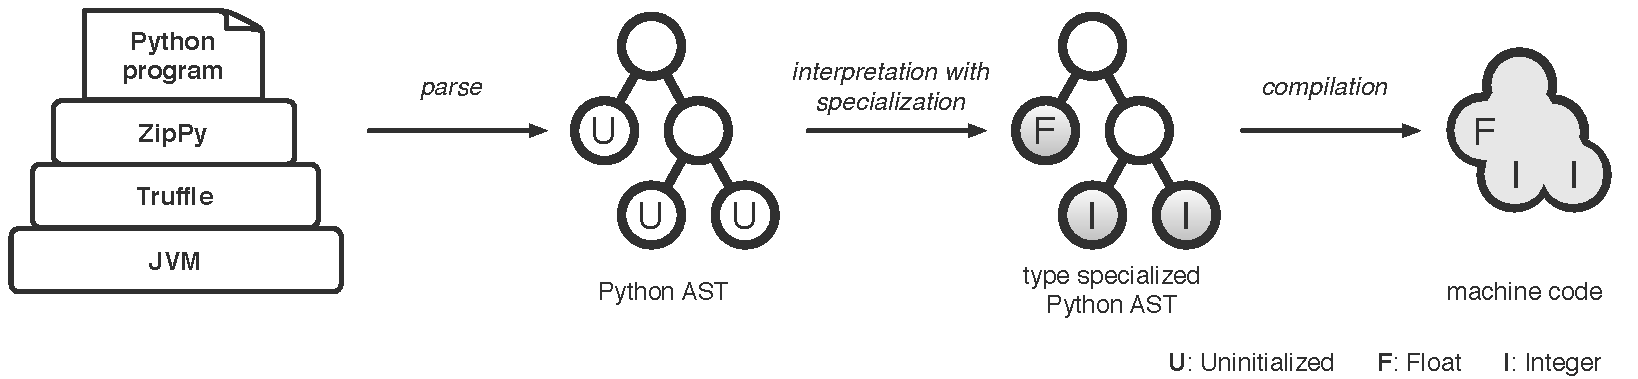
\includegraphics[scale=0.50]{figures/python-on-truffle.pdf}
\caption{Python on Truffle}
\label{fig:python_on_truffle}
\end{figure*}

In principle, ``everything'' can change at any moment in dynamic language programs.
This dynamic nature is the major impediment to ahead-of-time optimization.
In practice, however, programmers tend to minimize the rate of change, which makes the code highly predictable.
Types, for instance, typically remain stable between successive executions of a particular operation instance.
Deutsch and Schiffman report that speculative type specialization succeeds 95\% of the time in their classic Smalltalk-80 implementation~\cite{Deutsch1984}.

Truffle is a self-optimizing runtime system that makes it easy to perform type specialization for dynamic languages running on top of the Java Virtual Machines (JVM)~\cite{Wurthinger+13}.
It allows language implementers to implement their guest language by writing an AST interpreter using Java.
An interpreter written in this way enjoys low cost type specialization via automatic node rewriting~\cite{Wurthinger+12,Brunthaler2010inca,Brunthaler2010quickening}.
AST node rewriting collects runtime type information, and speculatively replaces the existing nodes with specialized and more efficient ones.
Subsequently, Truffle just-in-time compiles the specialized AST, written in Java, directly to machine code using the underlying Java compiler.
Upon a type mis-speculation, the specialized AST node handles the type change by replacing itself with a more generic one.
The node replacement triggers deoptimization from the compiled code and transfers execution back to the interpreter.
If the re-specialized AST stays stable, Truffle can again compile it to machine code.

Our system, ZipPy, is a full-fledged prototype Python 3 implementation built atop Truffle.
It leverages Truffle's type specialization feature and its underlying compilation infrastructure (see Figure~\ref{fig:python_on_truffle}).
This architecture helps ZipPy outperform Python implementations that either do not exploit runtime type specialization or lack a just-in-time compiler.
However, Truffle has no knowledge about specific high level guest language semantics, like generators in Python.
Further performance exploration of a guest language will mainly benefit from better insights on distinct features of the language and making better use of the host compiler based on those insights.
In this paper we focus on guest language level optimizations we added to ZipPy.

\section{ZipPy's Object Model Design}

\begin{figure}
\centering
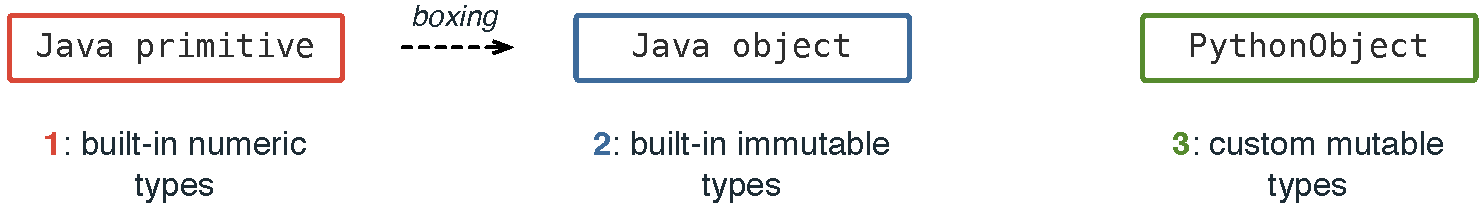
\includegraphics[scale=.34]{figures/three-data-representations}
\caption{Three data representations for Python objects}
\label{fig:three-data-representations}
\end{figure}

Python, although being a dynamic language, has a rich set of built-in types that are backed by C structs.
These types are inherently immutable.
Meaning that Python programs cannot add or remove attributes to or from it at runtime.
This feature separates it from languages like Ruby where you can monkey patch core classes of the language.
But it does offer opportunities for the language implementations like ZipPy to model immutable built-in types in a more efficient way.
Custom types defined in Python level are dynamic and mutable.
They can be as expected manipulated as map or dictionaries at runtime.
In the rest of this Section, we explain how we model them efficiently in ZipPy.

Python does offer more advanced features like metaclasses and attribute access customizations.
They do make the use of the language even more dynamic.
However, in this paper we donot focus on those advanced features.

\subsection{Multiple Data Representations}

ZipPy internally uses multiple data representations to model Python objects.
Figure~\ref{fig:three-data-representations} illustrates this design scheme.
The descriptions of each data representation are as follows:

\begin{enumerate}

\item \textbf{Built-in numeric types}
ZipPy, as explained in Chapter~, models some built-in numeric types, like \texttt{bool}, \texttt{int} and \texttt{float}, using Java primitives.
This approach helps to achieve Java level performance for arithmetic operations in ZipPy.
We refer types that has a Java primitive representation as \emph{unboxable}.
Each \emph{unboxable} numeric type in ZipPy has a corresponding \emph{boxed} representation using Java objects as a fall-back.
As shown in the Figure, a boxing operation will convert an instance of unboxable type, e.g., \texttt{int}, from its Java primitive representation to the boxed one.

\item \textbf{Built-in immutable types}
Similar to Jython, we implement Python built-in types including numeric types as regular Java classes.
In this way we map Python's built-in type hierarchy onto a Java class based type hierarchy.
Unlike custom types, all built-in types in Python are immutable meaning that user program cannot modify the attributes of an instance of a built-in type.
We take advantage of this immutability by modeling Python built-in types directly using Java classes on the JVM.

\item \textbf{Custom mutable types}
All custom or user defined types in Python are mutable.
That includes Python modules, custom type definitions written in Python and instances of custom classes.
We model them using still a regular Java object, an instance of \texttt{PythonObject} in ZipPy, to circumvent the performance overhead incurred by using a hash map.
ZipPy maps Python attribute accesses to field accesses on the \texttt{PythonObject} object.
We support attribute modifications by maintaining an object layout table for each Python object.
The object layout table keeps track of the memory offset for each attribute that is currently stored on the object.
We will discuss how we support attribute modifications on custom types in more detail in Section~.

\end{enumerate}

Although we model Python objects using different physical data representations, our approach preserve the semantics that every data in Python is an object.
ZipPy support object like operations on each of the data representations described above.
What differs our approach to the existing ones is that we do not treat all Python data types in the same way.
We try to pick the most efficient construct offered by the JVM that is suitable for implementing particular types in Python.
To be more specific, modeling Python numbers as Java primitives enables the best arithmetics performance achievable on the JVM.
Using Java object to model Python object brings the opportunity for ZipPy to close the performance gap of object operations between existing implementations of Python and Java.

\subsection{Modeling Custom Mutable Types}
\label{sec:ch5-custom-mutable-types}

\begin{figure}
\centering
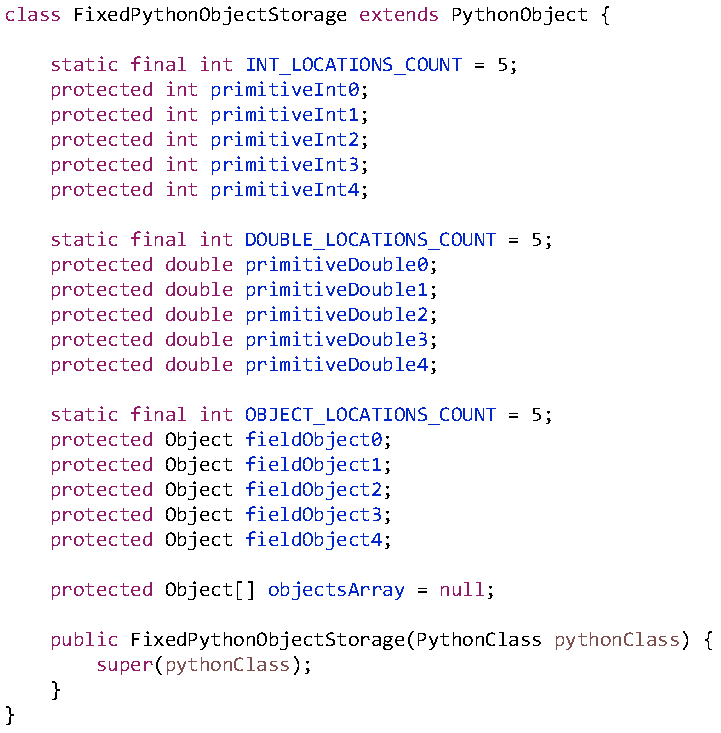
\includegraphics[scale=.7]{figures/fixed-python-object-code}
\caption{The implementation of \texttt{PythonObject}}
\label{ch5-fixed-python-object-code}
\end{figure}

\begin{figure}
\centering
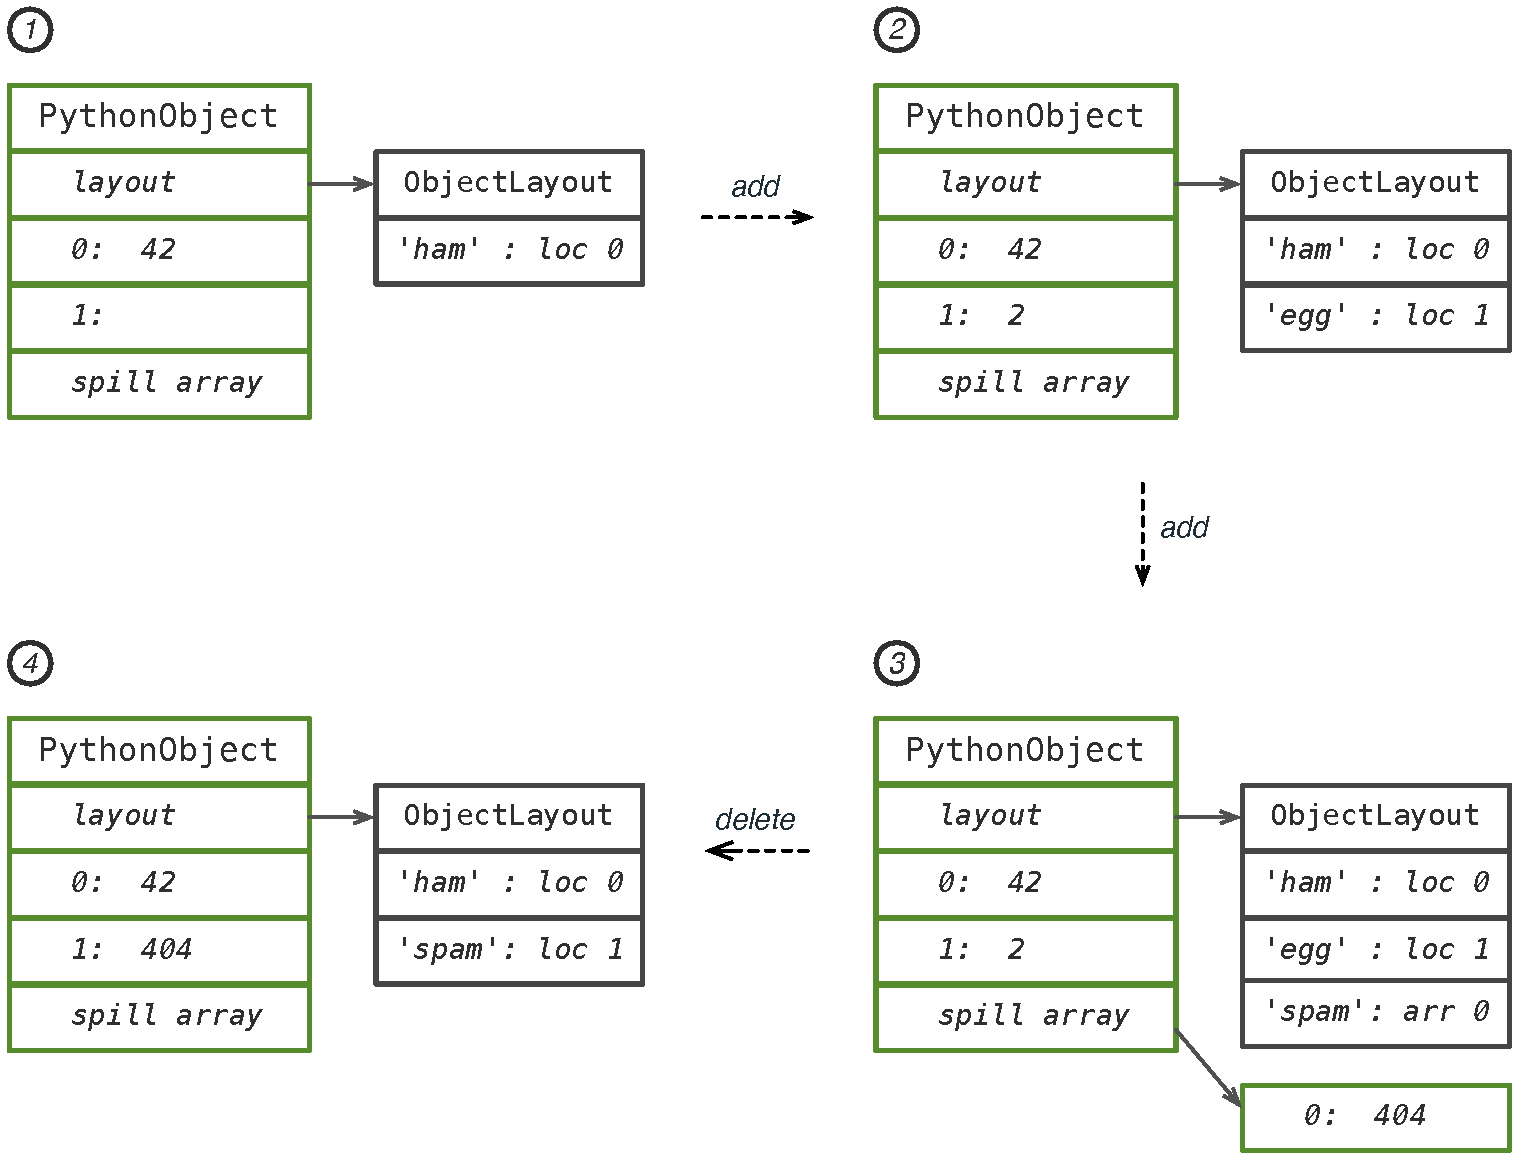
\includegraphics[scale=.34]{figures/mutable-object-layout-change}
\caption{Mutable object layout}
\label{ch5-mutable-object-layout-change}
\end{figure}

Python allows programmers to add, modify or delete attributes on an object during the execution of the program.
On the other hand, a Java object is fixed.
You can modify the value of a field, but cannot resize or change the layout of an object.
We support this dynamic feature of Python by implementing each Python object using a combination of a fixed \texttt{PythonObject} and a re-sizable object layout.

Figure~\ref{ch5-fixed-python-object-code} shows an implementation of \texttt{PythonObject} in ZipPy.
Each \texttt{PythonObject} has a fixed number of fields of both primitive and reference types to accommodate its attributes.
Each field on the object is a \emph{location}.
The object stores each of its attribute on a dedicated \emph{location}.
ZipPy tries to store an unboxed attribute in an unboxed location to avoid the overhead of boxing.
For instance, it tries to store a Java \texttt{int} in an \texttt{int} field when possible.
If all \texttt{int} fields are taken, it tries to stores the attribute in an \emph{boxed} location or an object field.
If no in-object location is available anymore (taken by other attributes), ZipPy will spill the incoming attribute to be stored in the additional object array (field \texttt{objectArray} in Figure~\ref{ch5-fixed-python-object-code}).
The additional object array gives the fixed \texttt{PythonObject} the ability to store more attributes than its own capacity by paying the price of another level of direction and possibly auto-boxing.

An object layout attached to a \texttt{PythonObject} keeps track of the list of attributes stored on the object as well as the location of each attribute.
It is essentially a table that maps the symbol of an attribute to its location.
The table records modifications made dynamically to the attributes of the object.
Figure~\ref{ch5-mutable-object-layout-change} illustrates how this process works by using a hypothetical Python object.
The layout of the shown object goes through the following stages:

\begin{enumerate}

\item The object initially has one attribute \textsf{ham} stored in location $0$ with the value $42$.

\item After adding the attribute \textsf{egg}, the object now has both \textsf{ham} and \textsf{egg} stored in location $0$ and $1$ respectively.

\item Since both in-object locations are taken, the object stores the new attribute \textsf{spam} in the spill array at the index $0$.
The rest of the layout remain unchanged.

\item The deletion of \textsf{egg} frees location $1$ on the object.
The object reassigns the newly available in-object location to \textsf{spam} to make sure that location assignments are optimal.
It also update the layout table to reflect the new changes.

\end{enumerate}

We simplified the structure of the Python object shown in Figure~\ref{ch5-mutable-object-layout-change} for brevity.
The actual algorithm for a layout update is more complicated.
Adding or deleting an attribute triggers a layout update.
The layout update tries to stores as many unboxed attributes in an unboxed location as possible.
The spill array allocation is lazy so that we only allocate the array when necessary.
During the layout update, ZipPy calculates the size of the additional spill array needed to accommodate all the attributes.
If it requires a spill array, we conservatively allocate an array that is just enough to store all the attributes.

In Python, attribute types can change at runtime.
An attribute type change also triggers a layout update.
Our current solution to handle such a type change is to assign a location that matches the most generic type of the attribute.
Once an unboxed attribute becomes boxed, we always assign a boxed location for this attribute in the future.

Our approach uses \texttt{PythonObject}s simply as a physical storage for the attributes of a Python object.
We detach the layout description of the Python object from its storage component.
This approach gives us the freedom to customize the behavior of attribute accesses in ZipPy without being restricted by Java's own object model.
Since we model class objects in the same way as we do for regular objects in Python, they enjoy the same potential performance benefit achieved by this design.

\subsection{Inline Caching for Attribute Accesses}

As explained in Section~\ref{sec:ch5-custom-mutable-types}, the layout table stores the location of object attributes.
Accessing an attribute requires looking up its location information from the layout table and then performing a memory read or write at the obtained memory location.
Since we implement the layout table using a hash map, the cost of accessing the table is as expensive as attribute accesses on a hash map based object.
However, ZipPy optimizes attribute accesses by caching attribute locations after a full layout table lookup.
This technique, inspired by previous research on virtual machines~\cite{Deutsch1984, Holzle+1991, Brunthaler2010inca}, amortizes the cost of accessing the same attribute on the Python objects of the same type.

\subsubsection{Attribute Access Dispatch Chain}
\label{sec:ch5-attribute-access-dispatch-chain}

\begin{figure}
\centering
\subfigure[Structure of \texttt{GetAttributeNode}]{
  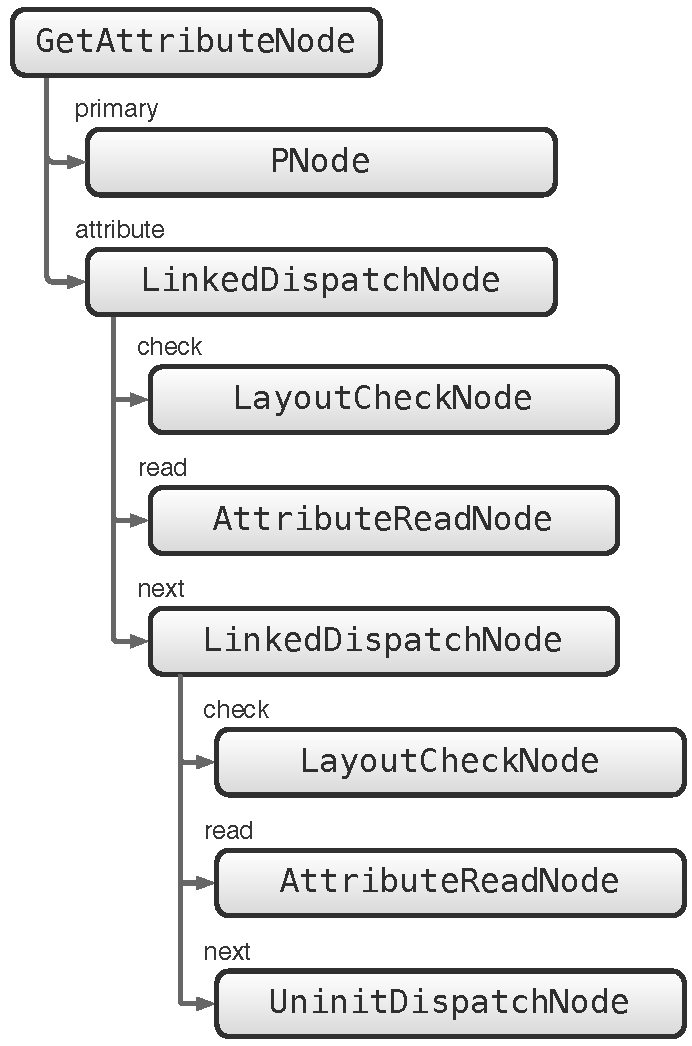
\includegraphics[scale=.4]{figures/get-attribute-node}
  \label{fig:ch5-get-attribute-node}
}
\subfigure[Structure of \texttt{SetAttributeNode}]{
  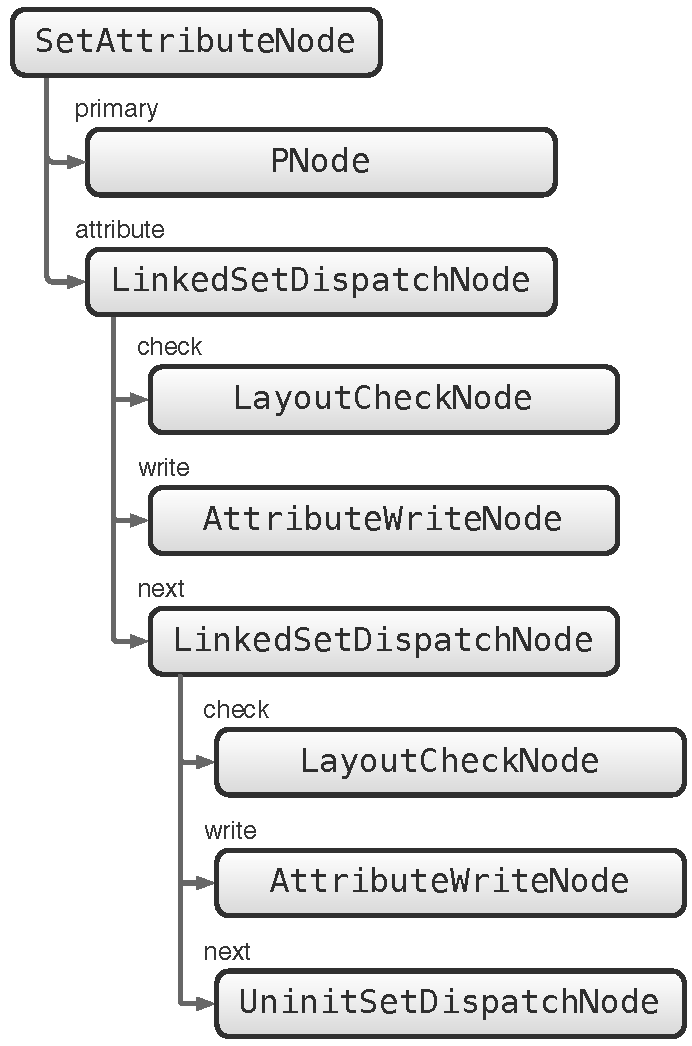
\includegraphics[scale=.4]{figures/set-attribute-node}
  \label{fig:ch5-set-attribute-node}
}
\caption{Attribute access dispatch chain}
\label{fig:ch5-attribute-access-dispatch-chain}
\end{figure}

Like the other operations, we model attribute accesses using AST nodes in ZipPy.
We model an attribute read operation using a \texttt{GetAttributeNode} and attribute write operation using a \texttt{SetAttributeNode}.
Figure~\ref{fig:ch5-attribute-access-dispatch-chain} illustrates the structure of these two nodes.
In each attribute access node, the \textsf{primary} child node represents the primary expression, the component precedes the period in Python's syntax.
The \textsf{primary} node evaluates to the Python object, on which we perform the attribute access.
The \textsf{attribute} nodes shown in both Figure~\ref{fig:ch5-get-attribute-node} and~\ref{fig:ch5-set-attribute-node} are dispatch chains that perform the actual read or write on the resolved object.

The attribute access dispatch chain is a linked list of dispatch nodes.
Each dispatch node has a \textsf{next} field that points to the next dispatch node except for the last one.
The chain forms a polymorphic inline cache with each node working as an individual cache entry.
Each entry stores the object layout and the location of a previously accessed attribute.
Upon a successive access to the attribute on a Python object sharing the same layout, the matching dispatch node performs a direct memory operation using the cached location.
In other words, a cache hit in the dispatch chain avoids executing the slow path lookup on the object layout.

ZipPy performs an attribute access operation in a number of steps.
It first evaluates the primary object, and passes the object to the dispatch chain.
The resolved primary object travels through the dispatch chain from the top to the bottom one dispatch node after another.
Each dispatch node tests the cached object layout against the one of the incoming object.
If the test returns a match, the dispatch node performs a fast read or write on the object and returns the result to the parent node if necessary.
Otherwise, execution falls to the next dispatch node on the chain until a cache hit occurs.
If no cache hit happened, the primary object reaches the uninitialized dispatch node at the end of the chain.
The uninitialized dispatch node, in this case, performs a full attribute access on the primary object including a lookup on its layout table.
Additionally, it also constructs a new cached dispatch node and inserts the new node between the uninitialized dispatch node and its predecessor.
The added entry increases the depth of the inline cache as well as the chance of a cache hit in the future.
However, if the cache depth reaches a certain threshold, ZipPy rewrites the entire dispatch chain to a single generic dispatch node that always perform a slow path lookup.

Each cache entry in the dispatch chain consists of a cluster of nodes coordinated by the dispatch node.
Besides the \textsf{next} field pointing to the next node, each dispatch node has a \texttt{LayoutCheckNode} as well as an \texttt{AttributeReadNode} or \texttt{AttributeWriteNode} (Figure~\ref{fig:ch5-attribute-access-dispatch-chain}).
The \textsf{check} node stores the cached object layout and performs the layout test.
The \textsf{read} or \textsf{write} node stores the cached attribute location and performs the actual memory read or write on the primary object.
When a layout update happens, ZipPy creates a new layout instance for the associated Python object.
ZipPy also signals the old layout as invalid, since it does not describe a valid layout for the associated object anymore.
Therefore, when performing a layout test the \texttt{LayoutCheckNode} also checks the validity of the cached layout.
If the cached layout become invalid, it throws an exception back to the parent node.
ZipPy handles the exception by removing the invalid cache entry from the dispatch chain.

\section{Flexible Object Layout Evolution}

\section{Evalutation}

\section{Conclusions}
This paragraph will end the body of this sample document.


\begin{acks}
  The authors would like to thank Dr. Yuhua Li for providing the
  matlab code of  the \textit{BEPS} method. 

  The authors would also like to thank the anonymous referees for
  their valuable comments and helpful suggestions. The work is
  supported by the \grantsponsor{GS501100001809}{National Natural
    Science Foundation of
    China}{http://dx.doi.org/10.13039/501100001809} under Grant
  No.:~\grantnum{GS501100001809}{61273304}
  and~\grantnum[http://www.nnsf.cn/youngscientsts]{GS501100001809}{Young
    Scientsts' Support Program}.

\end{acks}
